\documentclass[a4paper,11pt,BCOR10mm,oneside,headsepline]{scrartcl}
\usepackage{amsmath, mathtools}
\usepackage[ngerman]{babel}
\usepackage[utf8]{inputenc}

\usepackage{typearea, url}
\areaset{17cm}{26cm}
\setlength{\topmargin}{-1cm}
\usepackage{scrpage2}
\pagestyle{scrheadings}

\usepackage[T1]{fontenc}
\usepackage{beramono}
\usepackage{listings}
\usepackage[usenames,dvipsnames]{xcolor}
\usepackage{graphicx}
\usepackage{subcaption}

\ihead{HW4: CIS 631, Parallel Processing}
\ohead{\pagemark}
\chead{}
\cfoot{}

\begin{document}
	
	\begin{center}
		\textbf{\large Homework 4 Report}
	\end{center}\vskip1em
	
	\section{Test Environment}
	I tested my code on department's ix server. It has two sockets with AMD Opteron 6376 on each socket. Each CPU has 8 cores, 16 threads. So, there are 32 hardware threads in total.
		
	\section{Test Results}
	\subsection{Convergence Test Result for Tolerance of 1e-6, Using 32 Threads}
	\begin{table}[!htbp]
		\centering
		\begin{tabular}{|c|c|c|c|}
			\hline
			\textbf{Max Iteration} & \textbf{Time (seconds)} & \textbf{norm(b-A*x)} & \textbf{Converge}\\ \hline
			13,000                 & 25.515200    & 5.743765e-05 > 1e-6	& False        \\ \hline
			13,250                 & 27.533186   & 3.585957e-05 > 1e-6      & False  \\ \hline
			13,500                 & 26.683842    & 6.690461e-06 > 1e-6      & False  \\ \hline
			13,750                 & 26.256778    & 4.147648e-06 > 1e-6   	  & False    \\ \hline
			14,000                 & 27.199833    & 9.928136e-07					 & \color{red}True    \\ \hline
			15,000                 & 26.453255    & 9.593049e-07     			   & \color{red}True    \\ \hline
		\end{tabular}
		\caption*{Table 1. Convergence Test}
	\end{table}

	
	\subsection{Performance vs. Threads, Using Tolerance of 1e-6, 14,000 Max Iterations}
	\begin{table}[!htbp]
		\centering
		\begin{tabular}{|c|c|c|}
			\hline
			\textbf{Threads} & \textbf{Time} & \textbf{norm(b-A*x)} \\ \hline
			2                & 251.994506        &  9.512838e-07        \\ \hline
			4               & 127.116177    & 9.076329e-07         \\ \hline
			8               & 67.801198     &  9.583944e-07       \\ \hline
			16              & 39.024688   & 9.372702e-07         \\ \hline
			32               & 26.754807    & 9.147343e-07         \\ \hline
		\end{tabular}
		\caption*{Table 2. Performance Scaling for number of threads}
	\end{table}

	\begin{figure}[!htbp]
		\centering
		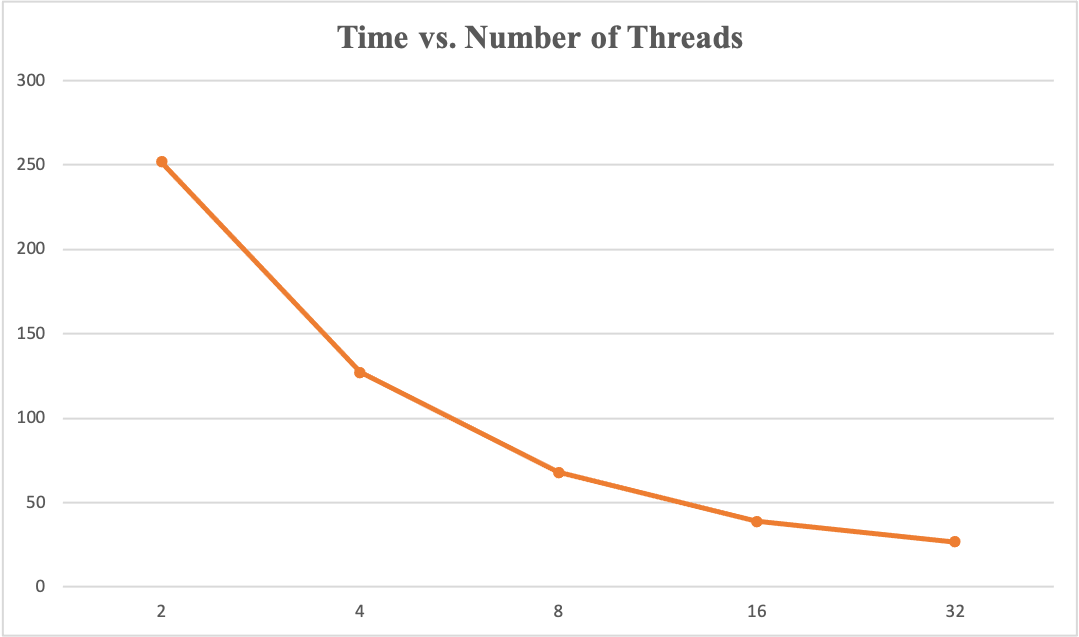
\includegraphics[scale=0.5]{plot1}
		\caption*{Figure 1. Performance Scaling for number of threads}
	\end{figure}
	
	\newpage
	\subsection{Function cg() without omp tasks vs. Function cg() with omp tasks}
	\begin{table}[!htbp]
		\centering
		\begin{tabular}{|c|c|c|}
			\hline
			\textbf{Threads} & \textbf{Time} & \textbf{norm(b-A*x)} \\ \hline
			2                & 262.271384    & 1.205389e-06         \\ \hline
			4                & 137.757589    & 9.571862e-07         \\ \hline
			8                & 77.193165     & 9.879008e-07         \\ \hline
			16               & 46.175155     & 9.082830e-07         \\ \hline
			32               & 37.390880     & 9.578399e-07         \\ \hline
		\end{tabular}
		\caption*{Table 3. cg() with omp tasks}
	\end{table}

	\begin{figure}[!htbp]
		\centering
		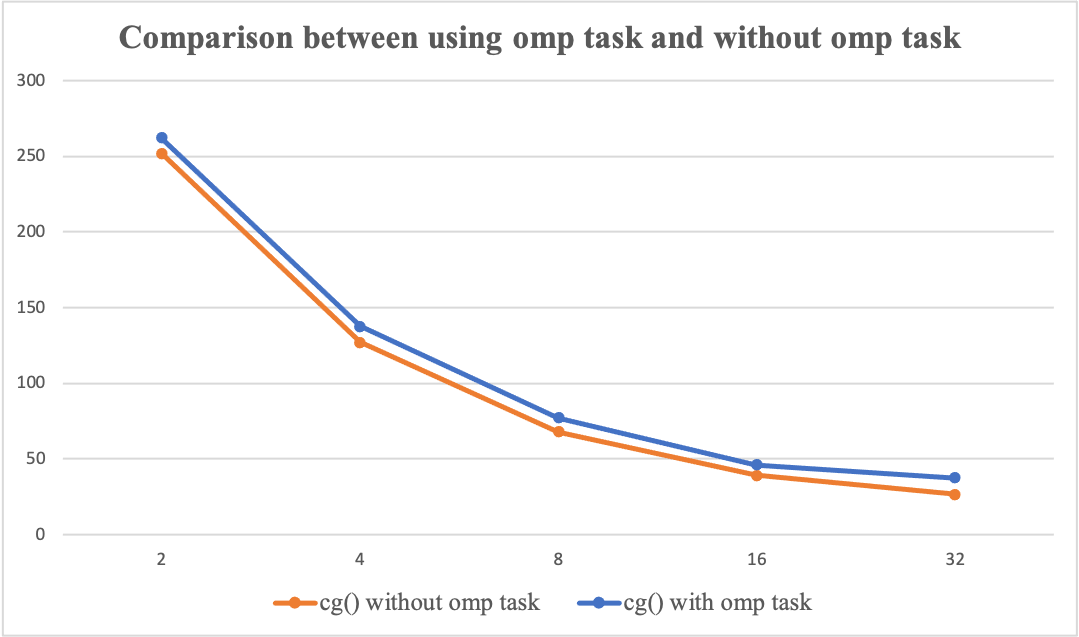
\includegraphics[scale=0.5]{plot2}
		\caption*{Figure 2. cg() without omp task vs. cg() with omp task}
	\end{figure}

	\section{Findings}
		\begin{itemize}
			\item For my implementation, CG does not converge for tolerance of 1e-6 when max iteration is below 14,000.
			\item The performance gain almost doubles when using double amount of threads.
			\item Since almost each step depends on the previous step in CG, there is not much opportunity for task-based parallelism. I attempted to add additional parallelization by using omp  tasks to simultaneously calculate:
			\begin{enumerate}
				\item x\_(k+1) = x\_(k) + alpha\_(k) * p\_(k)
				\item r\_(k+1) = r\_(k) - alpha\_(k) * A * p\_(k)
			\end{enumerate}
			However, by adding omp task will result approximately the same performance. This is most likely for two reasons. First, there is overhead for creating omp tasks. Second, most of the computational work has been done by vec\_add() in parallel.
		\end{itemize}
	
\end{document}